\begin{PROBLEM}
    رابطه صریح اعداد کاتالان را به دست آورید.
    \SOLUTION{
        \p
        می‌خواهیم سوال را به کمک دوگانه شماری حل کنیم. مسئله زیر را تعریف می‌کنیم:
        \p
    تعداد مسیر‌های از
    $A$
    به
    $B$
    در یک جدول
    $n\times n$
    را بیابید, به طوری که از نیمه سمت راست خارج نشویم و فقط حرکت‌های راست و بالا مجاز باشد.
    \begin{center}
    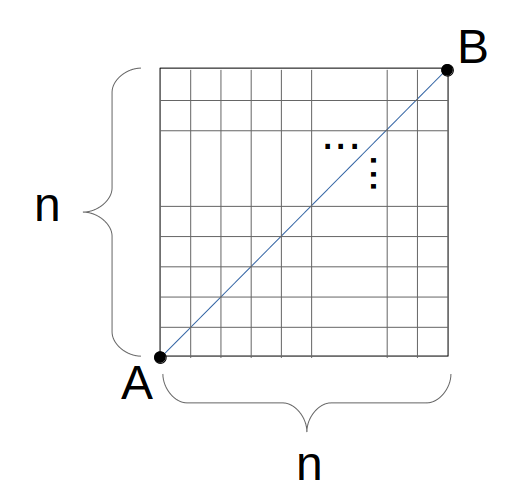
\includegraphics[totalheight=6cm]{ex2im1.png}
    \end{center}
        \p
        با کمی دقت متوجه می‌شویم که این مثال متناظر با مثال اول است, در واقع تعداد حرکات به سمت راست در اینجا معادل پرانتز باز و حرکات به سمت بالا متناظر با پرانتز بسته است. بنابراین تعداد جواب های این مسئله برابر اعداد کاتالان است.
        حال کافی است که این سوال را به روش غیر بازگشتی حل کنیم:
        \p
        سوال را با اصل متمم حل می‌کنیم:
        \begin{itemize}
            \item کل حالات:
            \p
            همان طور که در فصل شمارش بررسی شد, تعداد مسیر‌های
            از
            $A$
            به
            $B$
            برابر
            $$\binom{2n}{n}$$
            است.
            \item حالات نامطلوب: تعداد مسیر‌های 
            از
            $A$
            به
            $B$
            که در آن‌ها از قطر میانی عبور کنیم:
            \p
            ادعا می‌کنیم تناظری یک به یک بین تعداد این مسیر‌ها و تعداد مسیر‌های بین 
            $A$
            و
            $B$
            در یک جدول
            $n-1\times n+1$
            برقرار است.
            تناظر را به این صورت برقرار می‌کنیم که اولین حرکتی که از قطر میانی عبور کرده را در نظر می‌گیریم و تمام حرکات پس از آن را معکوس می‌کنیم  
            به این صورت که اگر حرکت به سمت بالا بود به سمت راست می‌رویم و اگر به سمت راست بود بالا می‌رویم:
            \begin{center}
                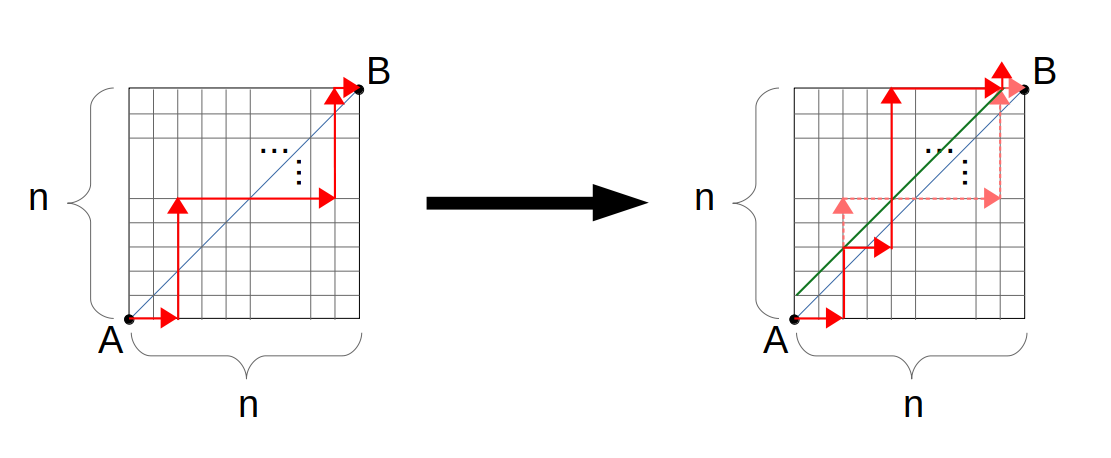
\includegraphics[totalheight=4cm]{ex2im2.png}
            \end{center}
            مشاهده می‌شود که با این تغییرات به یک مسیر از گوشه چپ پایین به گوشه راست بالا در یک جدول
            $n-1\times n+1$
            می‌رسیم.
            کافی است نشان بدهیم این فرایند به ازای هر جدول
            $n-1\times n+1$
            بازگشت پذیر است, برای این کار باید نشان دهیم که در هر مسیر از
            $A$
            به
            $B$
            در این جدول, نقطه‌ای وجود دارد که تعداد حرکات به سمت بالا تا آن نقطه بیشتر از تعداد حرکات به سمت راست است, برای اثبات این موضوع توجه کنید
            که در انتهای مسیر, تعداد حرکت‌های به سمت بالا دو تا بیشتر از تعداد حرکت‌های به سمت راست است, بنابراین قطعا نقطه‌ای وجود دارد که در آن نقطه برای اولین بار تعداد حرکات به سمت بالا از راست بیشتر شده است, برای معکوس کردن فرایند کافی است که از آن نقطه به بعد حرکات را معکوس کنیم.
            بنابراین تناظر یک به یک برقرار است و تعداد حالات نامطلوب برابر
            $$\binom{2n}{n-1}$$
            است. 
            \item حالات مطلوب:
            طبق اصل متمم برابر است با:
            $$\binom{2n}{n}-\binom{2n}{n-1}$$
        \end{itemize}
    }
    
\end{PROBLEM}